\documentclass[a4paper,oneside]{scrartcl} %twocolumn,
\usepackage[utf8]{inputenc} %für MAC: applemac; für Windows: latin1 statt utf8
\usepackage[T1]{fontenc}
\usepackage[ngerman]{babel}

\usepackage{amsmath}
\usepackage{amsfonts}
\usepackage{amssymb}

\usepackage{mathptmx}
\usepackage{microtype}
\usepackage[nice]{nicefrac}

\usepackage{booktabs}
\usepackage{graphicx}
\usepackage{hyperref}
\usepackage{wrapfig}

\setkomafont{captionlabel}{\upshape\bfseries}
\setkomafont{caption}{\itshape}


\title{Ultraschall}
\author{Robi Pedersen \and Simon Schmeißer}
\date{}

\begin{document}
\begin{titlepage}
  \maketitle
  \vfill
  \thispagestyle{empty}
  \begin{abstract}
    Hier sollte eine Zusammenfassung der Ergebnisse stehen. Der Umfang sollte dabei etwa 100 Wörte nicht überschreiten.
  \end{abstract}
\end{titlepage}

\tableofcontents
\clearpage
%*****************************************************************

\section{Aufgabenstellung}

\begin{enumerate}

\item Pockelseffekt: Für eine Pockelszelle bestimme man die Halbwellenspannung $U_{\lambda/2}$ und berechne daraus den elektrooptischen Koeffizienten $r_{41}$, indem man
\begin{enumerate}
	\item eine Spannung in Sägezahnform
	\item eine sinusmodulierte Gleichspannung
\end{enumerate}
an die Zelle anlegt.

\item  Faraday-Effekt: Für einen in einer stromdurchflossenen Spule befindlichen Schwerflintstab bestimme man die Verdet-Konstane mit Hilfe eines Halbschattenpolarimeters.

\end{enumerate}
\section{Theorie}

%Was ist Beugung(Einzelspalt, Gitter, Aperturfunktion, Sinusgitter, Fouriertrafo)
%Laser (nur Eigenschaften)

\subsection{Beugung}

\subsubsection{Allgemeine Definition}

Als Beugung bezeichnet man das Ph\"anomen, dass Licht, welches durch begrenzende \"Offnungen oder an begrenzenden Kanten vorbeil\"auft, von seiner urspr\"unglichen Richtung abgelenkt wird. Hinter dem Hindernis \"uberlagern sich die Teilwellen gem\"a\ss dem Huygenschen Prinzip, welches besagt, dass jeder Punkt einer Wellenfront eine neue Welle induziert. Diese \"uberlagern sich dann und die daraus resultierenden Interferenzerscheinungen werden als Beugung bezeichnet.

\subsubsection{Das Kirchhoff'sche Beugungsintegral}

\begin{figure}[H]
	\centering 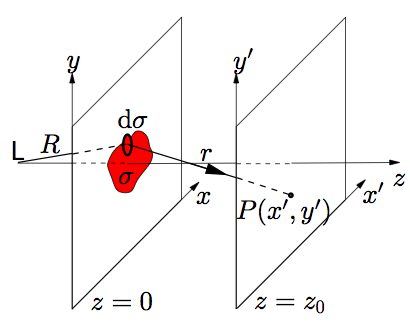
\includegraphics[width=0.5\textwidth]{Bilder/Beugungsintegral.jpg}
	\caption{Zum Kirchhoffschen Beugungsintegral}
\end{figure}

Licht mit der Amplitude $E_\sigma$, welches auf die Blenden\"offnung $\sigma$ f\"allt, hat im Punkt $P$ auf dem Schirm hinter der \"Offnung die Amplitude: $$dE_P = C\frac{E_\sigma \cdot d\sigma}{r}e^{-ikr}$$
($C$ ist hier ein Proportionalit\"atsfaktor)\\
Betrachtet man die Beitr\"age aller $d\sigma$, so erh\"alt man das Fresnel-Kirchhoffsche Beugungsintegral:
$$E_P=\iint C\cdot E_\sigma \cdot \frac{e^{-ikr}}{r}dxdy$$

Dieses Integral kann man nun mit der Fraunhofer-N\"aherung als Fourierintegral umwandeln. Die Fraunhofer-N\"aherung ist eine Fernfeldn\"aherung; die Spaltgr\"o\ss e wird als klein angenommen und die Lichtquelle als sehr weit entfernt. Mit diesen Vereinfachungen wird das Integral zu:

$$ E(x',y') = A(x',y',z_0)\cdot \iint E_{ein}(x,y)\cdot g(x,y)\cdot \exp(-i2\pi(x'x+y'y)/(\lambda z_0)) dxdy $$

und es gilt der Zusammenhang:

$$ E(x',y',z_0) = F(u,v) \cdot A(x',y',z_0)$$

wobei \begin{itemize}
\item $F(u,v)$ das Fourierintegral der Funktion $f(x,y) = g(x,y)\cdot E_{ein}(x,y)$
\item $g(x,y)$ die Aperturfunktion der \"Offnung
\item $A(x',y',z_0)=\frac{e^{-ikz_0}}{i\lambda z_0}\cdot e^{i\pi (x'^2 + y'2) / \lambda z_0}$ und $|A|^2 =1$
\end{itemize}

Somit folgt f\"ur die Intensit\"at:

$$I \sim |E|^2 = \iint g(x,y)\cdot e^{ikr} dxdy$$


\subsubsection{Anwendungen}

\begin{enumerate}
 
\item Beugung am Einzelspalt


\begin{minipage}{0.6\textwidth}
Die Aperturfunktion am Einzelspalt (unter Vernachl\"assigung der Begrenzung in y-Richtung) lautet
$$ g(x) = \begin{cases} 
	1 & \text{, falls} -\frac{b}{2}<x<\frac{b}{2}\\
	0 & \text{, sonst}
     \end{cases}$$
Man erh\"alt durch Ausrechnen des Beugungsintegrals folgende Abh\"angigkeit f\"ur die Intensit\"at:
$$ I \sim \left(\frac{\sin(\beta)}{\beta}\right)^2 $$
\end{minipage}
\begin{minipage}{0.4\textwidth}
	\begin{center}
		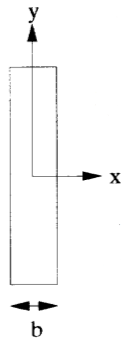
\includegraphics[width=0.35\textwidth]{Bilder/Einzelspalt.jpg}
	\end{center}
\end{minipage}

Hier ist $\beta = \frac{k}{2b}\sin(\theta)$ und $\theta$ der Einfallswinkel auf dem Schirm vom Ursprung des Spaltes aus.

\item Beugung am Gitter

\begin{minipage}{0.6\textwidth}
Ein Gitter besteht aus N Einzelspalten nebeneinander angeordnet. Alle Spalten haben idealerweise die Breite $b$ und die Distanz $K$ voneinander in $x$-Richtung.
\end{minipage}
\begin{minipage}{0.4\textwidth}
	\begin{center}
		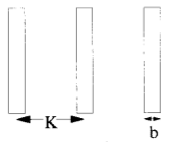
\includegraphics[width=0.7\textwidth]{Bilder/Gitter.jpg}
	\end{center}
\end{minipage}



\end{enumerate}
















\subsection{Ultraschallzelle}
Die Ultraschallzelle nach Karolus und Helmberger \cite{Karolus} besteht aus zwei Schwingquarzen, welche entgegengesetz schwingen und dadurch eine stehende Welle erzeugen. Diese wird dann von Isooktan übertragen, wobei sich dessen Dichte periodisch ändert. Dadurch ändert sich der Brechungsindex lokal \cite{Raman}: 
\begin{equation}
 \mu \left( x \right) = \mu_0 - \mu sin \frac{2 \pi x}{ \lambda^*}
\end{equation}
mit $x$ der Position entlang des Wellenvektors, $\mu_0$ dem Brechungsindex im ungestörten Zustand, $\mu$ der maximalen Abweichung davon und $\lambda^*$ der Wellenlänge des Schalls. Das Isooktan bildet somit ein sinusförmiges Phasengitter, d.h. kohärentes Licht
\begin{equation}
 A e^{i \omega t}
\end{equation}
das senkrecht auf das Bad trifft, hat nach Durchquerung einen Phasenversatz
\begin{equation}
 A e^{i \omega \left( t - L \frac{\mu \left( x \right)}{c} \right)}
\end{equation}
der ebenfalls sinusförmig ist ($L$ ist hierbei die Breite des Bades). 


Raman-Nath-Theorie(Besselfunktionen)

\section{Versuchsbeschreibung}

\subsection{Versuchsaufbau}
\begin{figure}[h]
\centering 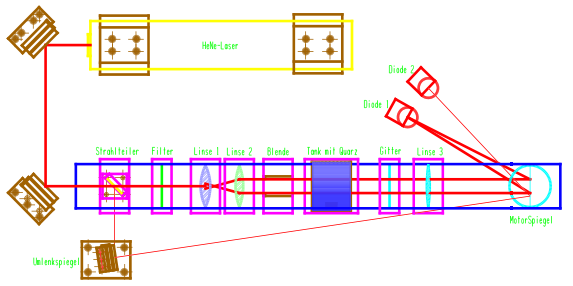
\includegraphics[width = \textwidth]{Bilder/Aufbau.jpg}
\caption{Schematischer Versuchsaufbau}
\end{figure}



\subsection{Durchf\"uhrung}

Mit einem He-Ne Laser, der monochromatisches Licht der Wellenl\"nge $\lambda = 6328 \mathring{A}$ abstrahlt, untersuchen wir das Beugungsph\"anomen an verschiedenen Gittern und bestimmen daraus die Gitterkonstanten bzw. Aperturfunktionen dieser Gitter. Bei einem Ultraschallgitter versuchen wir au\ss erdem die Schallwellenl\"ange in einer Isooktan-L\"osung herauszufinden und vergleichen unsere Messergebnisse mit der Raman-Nath-Theorie.

\subsubsection{Sinusgitter}

Wir richten den Laserstrahl senkrecht auf das Sinusgitter ohne Aufweitung und ohne Kollimationslinse, da bei diesem Gitter die 0. und die 1. Ordnung problemlos unterscheidbar sind. Auf einem Schirm hinter dem Gitter kann man das Beugungsmuster direkt beobachten und somit die Gitterkonstante bestimmen.

\subsubsection{Amplitudengitter}

Die H\"ohen der Linsen werden korrekt justiert und der Strahl wird durch Autokollimation auf Parallelit\"at \"uberpr\"uft. Dann wird der Drehspiegel eingesetzt und die Dioden werden so eingestellt, dass sie die maximale Signalintensit\"at aufnehmen k\"onnen. Schlussendlich eichen wir die Zeitachse des Oszilloskopenbildes anhand des Gitters "R". Anhand der Distanzen (Zeiten) zwischen dem Hauptmaximum und aller sichtbaren Beugungsordnungen auf dem Oszilloskop f\"ur alle Gitter, bestimmen wir durch lineare Regression die Umrechnungformel von Zeiten in Brechungswinkel.

\subsubsection{Aperturfunktion}

\clearpage

\section{Messwerte}

\section{Auswertung}

\section{Zusammenfassung}



\clearpage
%*****************************************************************
\appendix
Hier könntet ihr noch Bilder und Tabellen anhängen.
\clearpage


%*****************************************************************
\bibliographystyle{alphadin} 
\bibliography{bib}


\end{document}
